% !TEX root = mythesis.tex

%==============================================================================
\chapter{Data Reduction}
\label{sec:data_reduction}
%==============================================================================
In the following section, the underlying data shall be reduced and corrected for the various effects and contamination sources explained in Section \ref{sec:background}. Data from eRASSX is utilized for for all TMs (1-7) using \textit{eROSITA} pipeline processing version c010. The galaxy group NGC1550 is located in skytile 065087. In addition, the surrounding skytiles 062084, 062087, 062090, 065084, 065090, 068084, 068087, 068090 are used to encompass regions up to \(\sim 3R_{200}\). The data reduction is performed with the software HEASoft version XXX and the extended Science Analysis Software System (eSASS 4DR1). Images were created using astropy.
%
\section{Raw photon images}
Before the data reduction process, raw photon images for all combined skytiles and TMs are presented across the following energy bands: \SIrange{0.2}{2.3}{\kilo\electronvolt}, \SIrange{2.3}{6.0}{\kilo\electronvolt}, and \SIrange{6.0}{9.0}{\kilo\electronvolt}. The skytiles were combined using the \textit{eSASS} task \texttt{evtool}, with no additional parameters applied to reveal all inherent deficiencies in the raw images. The raw photon images are presented in \ref{fig:raw_photon_images}. As observed, most cluster emission is concentrated in the lower energy band, making it the focus for detecting emission structures. In this analysis, the \SIrange{0.2}{2.3}{\kilo\electronvolt} energy band is used. Due to the light-leak in TM9, however, the energy range is restrictated to \SIrange{0.8}{2.3}{\kilo\electronvolt}, while for TM8 it remains \SIrange{0.2}{2.3}{\kilo\electronvolt}. Hereafter, this TM-dependent energy band will be referred to as the \enquote{soft band} and the \SIrange{6.0}{9.0}{\kilo\electronvolt} energy range as the \enquote{hard band}. 
\begin{figure}[htbp]
    \centering
    \begin{subfigure}{0.32\textwidth}
        \centering
        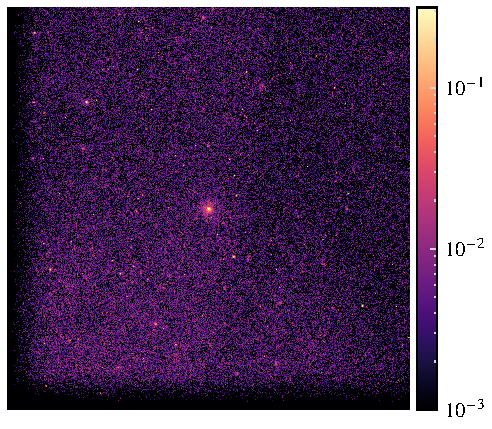
\includegraphics[width=\textwidth,height=\textwidth,keepaspectratio]{data_reduction/combined_tiles_0_raw_0.2-2.3keV.pdf}
        \caption{\SIrange{0.2}{2.3}{\kilo\electronvolt}}
        \label{fig:low_energy}
    \end{subfigure}
    \hfill
    \begin{subfigure}{0.32\textwidth}
        \centering
        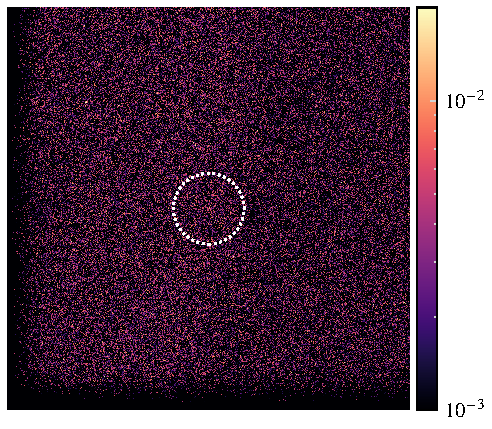
\includegraphics[width=\textwidth,height=\textwidth,keepaspectratio]{data_reduction/combined_tiles_0_raw_2.3-6.0keV.pdf}
        \caption{\SIrange{2.3}{6.0}{\kilo\electronvolt}}
        \label{fig:mid_energy}
    \end{subfigure}
    \hfill
    \begin{subfigure}{0.32\textwidth}
        \centering
        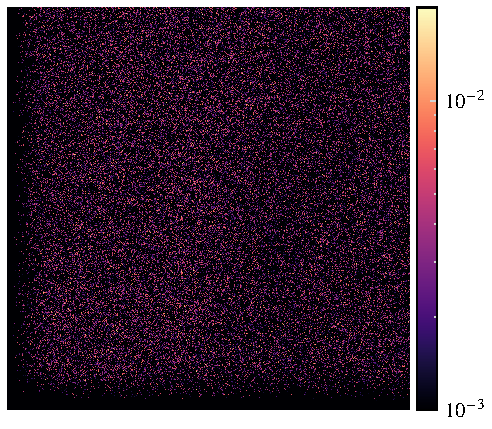
\includegraphics[width=\textwidth,height=\textwidth,keepaspectratio]{data_reduction/combined_tiles_0_raw_6.0-9.0keV.pdf}
        \caption{\SIrange{6.0}{9.0}{\kilo\electronvolt}}
        \label{fig:high_energy}
    \end{subfigure}
    \caption{Raw photon images from TM0 of all combined skytiles centered around NGC1550, displayed in the energy bands \SIrange{0.2}{2.3}{\kilo\electronvolt}, \SIrange{2.3}{6.0}{\kilo\electronvolt}, and \SIrange{6.0}{9.0}{\kilo\electronvolt}, with Gaussian smoothing of 4 pixels applied. The colorbar represents (smoothed) photon counts. Most of the cluster emission is visible in the lower energy band (\SIrange{0.2}{2.3}{\kilo\electronvolt}). A noticeable count drop on the right side of the images is evident and will be addressed through the exposure map correction detailed in Section X.}
    \label{fig:raw_photon_images}
\end{figure}
%
\section{Image filtering}
Each skytile is cleaned individually using \texttt{evtool} with \texttt{pattern=15} to select all event patterns and \texttt{flag=0xc00fff30} to remove bad pixels and CCD corners. Subsequently, soft proton flares are identified and mitigated through the following process: the \texttt{flaregti} task is used to generate light curves with \SI{20}{\second} time bins in the energy range of \SIrange{5}{10}{\kilo\electronvolt}. A \(3\sigma\) threshold is determined; time intervals exceeding this threshold indicate elevated count rates likely due to soft proton flares. The task \texttt{flaregti} is then rerun using this threshold to establish good-time-intervals (GTIs) excluding these flare periods, which are applied using \texttt{evtool} with the \texttt{gti="FLAREGTI"} parameter. All SPF-filtered and cleaned skytiles are combined into a single TM0 photon image using \texttt{evtool}. Hereafter, these combined images shall be referred to as \enquote{filtered}. The \texttt{evtool} task with the \texttt{telid} parameter is also used to split the filtered photon images into individual filtered images for each TM, as needed for subsequent steps.
%
\section{PIB-Correction}
Subtracting the particle-induced background (PIB) from the combined filtered photon image is necessary. The following  approach is based on extensive studies of the \textit{eROSITA} FWC data conducted by Dr. F. Pacaud, as utilized for example in \cite{Reiprich2021}.  The PIB is modeled for each TM using filter wheel closed (FWC) data. Due to the minimal spatial variation of the PIB, this modeling utilizes the flat exposure map created with the \textit{eSASS} task \texttt{expmap}. Furthermore, given the negligible spectral variation, the counts \(H_\text{obs}\) in the hard band, where PIB counts dominate, is used to estimate the PIB contribution in the soft bands by multiplication with the ratio \(R\) of the number of FWC counts in the soft band \(S_{\text{FWC}}\) to the hard band \(H_\text{FWC}\). A background map for each TM is then generated by applying this factor to the flat exposure map, normalized to 1 by dividing by the sum of all pixel values (norm. exposure map). Hence, the PIB map of a given TM is given by
\begin{align*}
    \text{PIB map}_\text{TM} = H_\text{obs}R\cdot\bigl(\text{norm. exposure map}\bigr)
\end{align*}
PIB corrected image are obtained by subtracting the PIB map of each TM from the respective filtered photon image. The complete image for TM0 is obtain by co-adding all PIB corrected images. Furthermore, individual background maps are also co-added to form a complete PIB map, which can be found in Appendix \ref{sec:appendix_a_pib_map}. Figure \ref{fig:comparison_of_spf_and_filtered} compares the TM0 filtered image before and after PIB correction.
\begin{figure}[htbp]
    \centering
    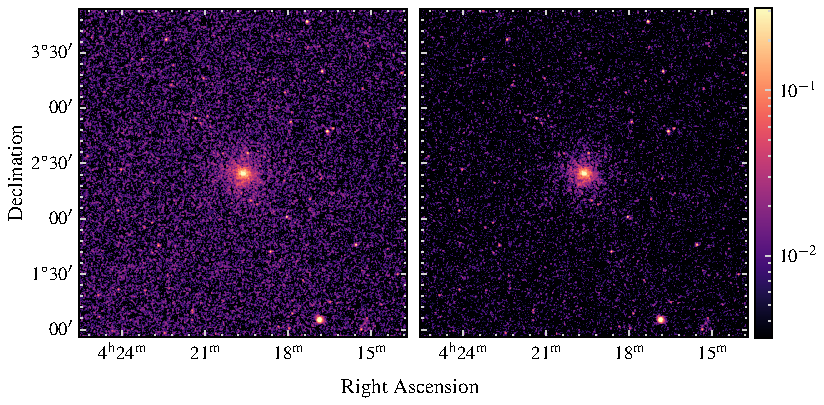
\includegraphics{data_reduction/comparison_SPF_filt_PIB_corr_0.pdf}
    \caption{Photon images of NGC1550 in the soft band with Gaussian smoothing of \(4\) pixels. Left: SPF-filtered and cleaned image. Right: image after PIB correction. The colorbar represents smoothed counts, same scalling is used for comparison.}
    \label{fig:comparison_of_spf_and_filtered}
\end{figure}
\section{\(N_\text{H}\) Absorption Correction}
As discussed in Section \ref{sec:background}, X-ray absorption by the ISM must be considered. At higher energies (\(\gtrsim \SI{0.28}{\kilo\electronvolt}\)), as is relevant for this analyis, metals from stellar processes play a significant role. Assuming solar metallicity, the hydrogen column density along the line of sight can serve as an indicator of the amount of absorbing material. This involves utilizing the total hydrogen column density, including all its states neutral, molecular, or ionized. A cutout of the HI4PI all sky survey is therefore reprojected on to the relevant skytiles.  







